\section{NetworkHandler and entities}
Every object that sends/receives data does so via the \emph{NetworkHandler}.
The \emph{NetworkHandler} is a class that acts as an interface between clients and the server.
Mostly, it is used by \emph{NetworkEntities}, as seen in Figure \ref{fig:networkHandler}.

\begin{figure}[H]
\centering
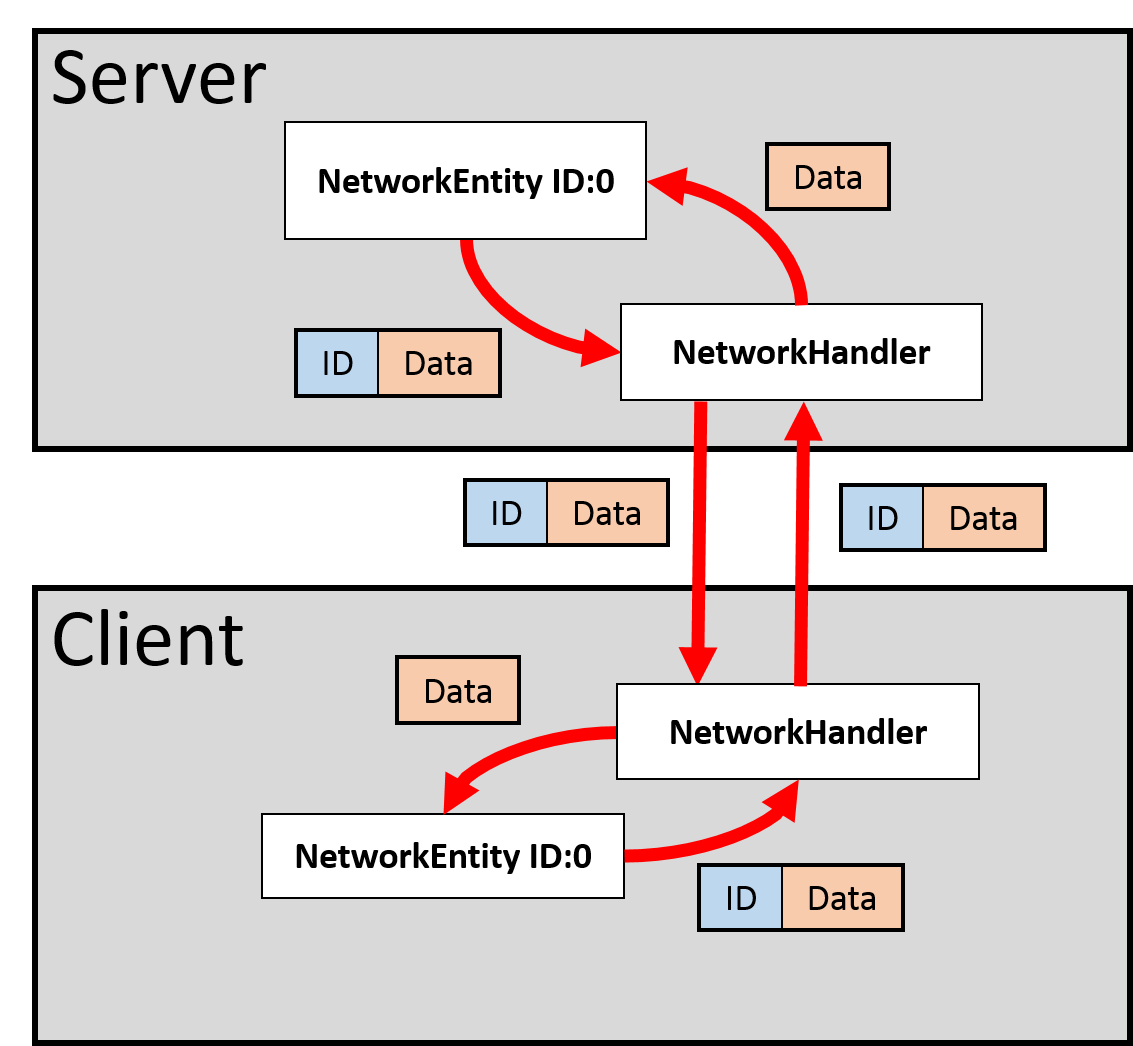
\includegraphics[width=\textwidth]{figures/network/networkHandler}
\caption{The NetworkEntities use the NetworkHandler to communicate.}
\label{fig:networkHandler}
\end{figure}

A \emph{NetworkEntity} comes in a client-version and a server-version.
They both inherit from a shared base, as illustrated in Figure \ref{fig:networkEntity}.
The shared base contains the input, the state and an id.

\begin{figure}[H]
\centering
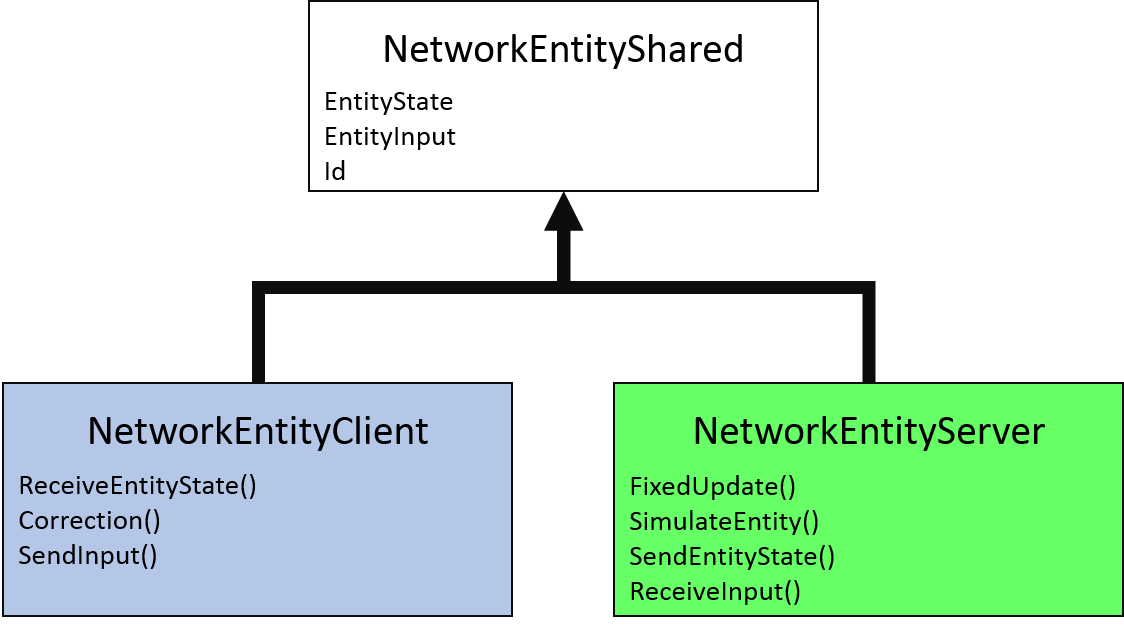
\includegraphics[scale=0.6]{figures/network/networkEntity}
\caption{Architecture of NetworkEntities.}
\label{fig:networkEntity}
\end{figure}

The timeline in Figure \ref{fig:clientServerEntities} shows how an entity is spawned.
On the server, the entity is given a \emph{NetworkEntityServer} and on the client it is given a \emph{NetworkEntityClient}.
Each entity spawned into the game world is given a unique id, which is the same for that entity on both the server and the client.
This id enables the \emph{NetworkHandler} to know which entity to deliver network messages to.

\begin{figure}[H]
\centering
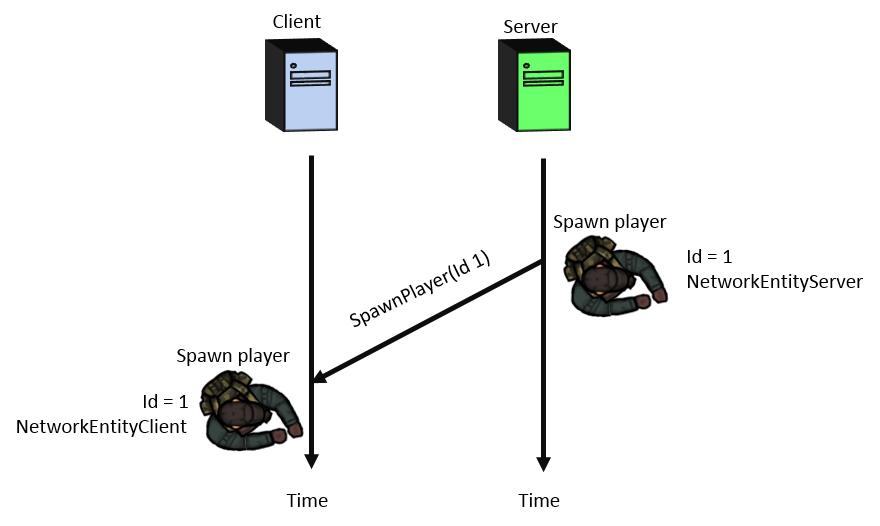
\includegraphics[width=\textwidth]{figures/network/clientServerEntities}
\caption{Timeline of server spawning a Player. The server spawns a Player and assigns an ID to it. The server then sends a message to the clients to spawn a Player with the same ID. Character Art by rileygombart\cite{artist}.}
\label{fig:clientServerEntities}
\end{figure}

The \emph{NetworkEntityClient} then sends a message to the corresponding \emph{NetworkEntityServer} with the input given by the player.
The \emph{NetworkEntityServer} receives this input and includes it in the game simulation.
Afterwards the \emph{NetworkEntityServer} will then send a message to the corresponding \emph{NetworkEntityClient} with its new state.
Upon receiving a new state, the \emph{NetworkEntityClient} then corrects itself to match the new state.
